%sagemathcloud={"latex_command":"lualatex -synctex=1 -interact=nonstopmode Greek.tex"}
\documentclass[b5j,8pt,twocolumn]{ltjsarticle}
\usepackage{amsmath} 
\usepackage{graphicx} 
\usepackage{tikz} 
\usepackage{tikz-cd} 
\usepackage{tikz-qtree}
\usepackage{wrapfig} 
\usepackage{tabularx} 
\usepackage{begriff} 
\usepackage{ascmac} 
\usepackage{multirow,bigdelim} 
\usepackage{blindtext} 
\usepackage[LGR,T1]{fontenc} 
\usepackage{pictexwd,dcpic}
\usepackage[LGR,T1]{fontenc}
\usepackage[OT2,OT1]{fontenc} \newcommand\cyr
{
\renewcommand\rmdefault{wncyr} \renewcommand\sfdefault{wncyss} \renewcommand\encodingdefault{OT2} \normalfont
\selectfont
}
\DeclareTextFontCommand{\textcyr}{\cyr} \def\cprime{\char"7E } \def\cdprime{\char"7F } \def\eoborotnoye{\char’013} \def\Eoborotnoye{\char’003}
\reserveinserts{28}
\newcommand{\textgreek}[1]{\begingroup\fontencoding{LGR}\selectfont#1\endgroup}
\makeatletter
\def\ruby#1#2{\leavevmode\vbox{%
\baselineskip\z@skip\lineskip.25ex
\ialign{##\crcr\rubyfont\hfill#2\hfill\crcr
\hfill#1\hfill\crcr}}}
\newcount\gpten % (global) power-of-ten -- tells which digit we are doing
\countdef\rtot2 % running total -- remainder so far
\countdef\LDscratch4 % scratch
\newcommand{\textgreek}[1]{\begingroup\fontencoding{LGR}\selectfont#1\endgroup}

\title{おんなのこLinux原稿 その1($\beta$-2版)\\
- アリストテレスとオブジェクト指向プログラミング -}
\author{三番街公爵(Marques de Third)}
\date{
平成27年11月13日
 }

\begin{document}
\maketitle

\vspace{10cm}

おんなのこLinux 原稿その1\copyright (2015) 横田 博史著\par

この著作の内容による損害に対し

著者は一切の責任を負いません.
\clearpage
\newpage
\setcounter{page}{1}



\section{はじめに}

ギリシャといえば今や国家の財政破綻や中近東の難民の大波ばかりが目立つ
状態ですが, ギリシャからさまざまな恩恵を我々は受けています. まず怪しいもの
にBLとGLの同性愛, そうでなく重要なものとしては神話, 詩や悲劇, 彫像や建築,
 そして哲学や論理学\footnote{論理学を発明・発展させた民族は他にガンジス文明
しかないのです!}, 数学や天文学, そして医術等の科学全般といったものでしょうか. 
\newline

BLでは古代ギリシャの都市国家テーバイ(\textgreek{J'hbai})の
「\textbf{神聖隊(\textgreek{>Ier'o L'oqos})}」\footnote{某アイドルグループ
とその所属事務所とは傾向等が似ていても違います.}を語らずにはいられません.
 この神聖隊は「\textbf{やおいのか硬いのか判らない}」のですが, 実際は
「\textbf{とてもやおく}」て「\textbf{とても硬い}」のです. まず
「\textbf{やおい}」ことについて語るなら, 神聖隊は恋人同士(勿論, 男同士です!)
150組, 300名で編成されていたそうです. 「\textbf{硬さ}」について語るなら,
 彼等は「\textbf{精鋭歩兵部隊}」だったのです. こういった部隊を編成した理由
が, 恋人に無様な自分を見せたり危険な目に合わせる訳にも行かないがため, 勇敢
に戦うだろうとかで, 実際, テーバイをギリシャの覇権国家にする要因の一つに
なったと云います. 
\newline

\begin{wrapfigure}{l}{5cm}
\includegraphics[width=5cm]{arno_breker_kameradschaft.pdf}
\caption{ブレーカー:戦友}
\label{fig:breker2}
\end{wrapfigure}

ところで神聖隊はマケドニア王国とギリシャの覇権を巡ってカロネイアの戦い
で王太子時代のアレクサンダー大王(\textgreek{>Al'exandros G'})率いる騎兵隊と
マケドニア式ファランクスの為に254名(丁度偶数!)が討死するという壊滅的打撃を
受けます. マケドニア王ピリッポス2世(\textgreek{F'ilippos B'})は彼等の亡骸を
見て涙したとのことですが, 戦いの半ば以降は図\ref{fig:breker2}の有様だった
ことでしょう. ちなみにこのレリーフはナチス時代の人気彫刻家ブレーカー
(Arno Breker)\footnote{ブレーカーの戦時中の手記が出版されていますが,
 その内容は非常にまともです.}のレリーフで, この味わいも現実の突撃隊の同性愛
を含む酒池肉林に変幻するというものでしょうか? たとえば図\ref{fig:rrevue}の
ように... 

\begin{figure}[htbp]
\begin{center}
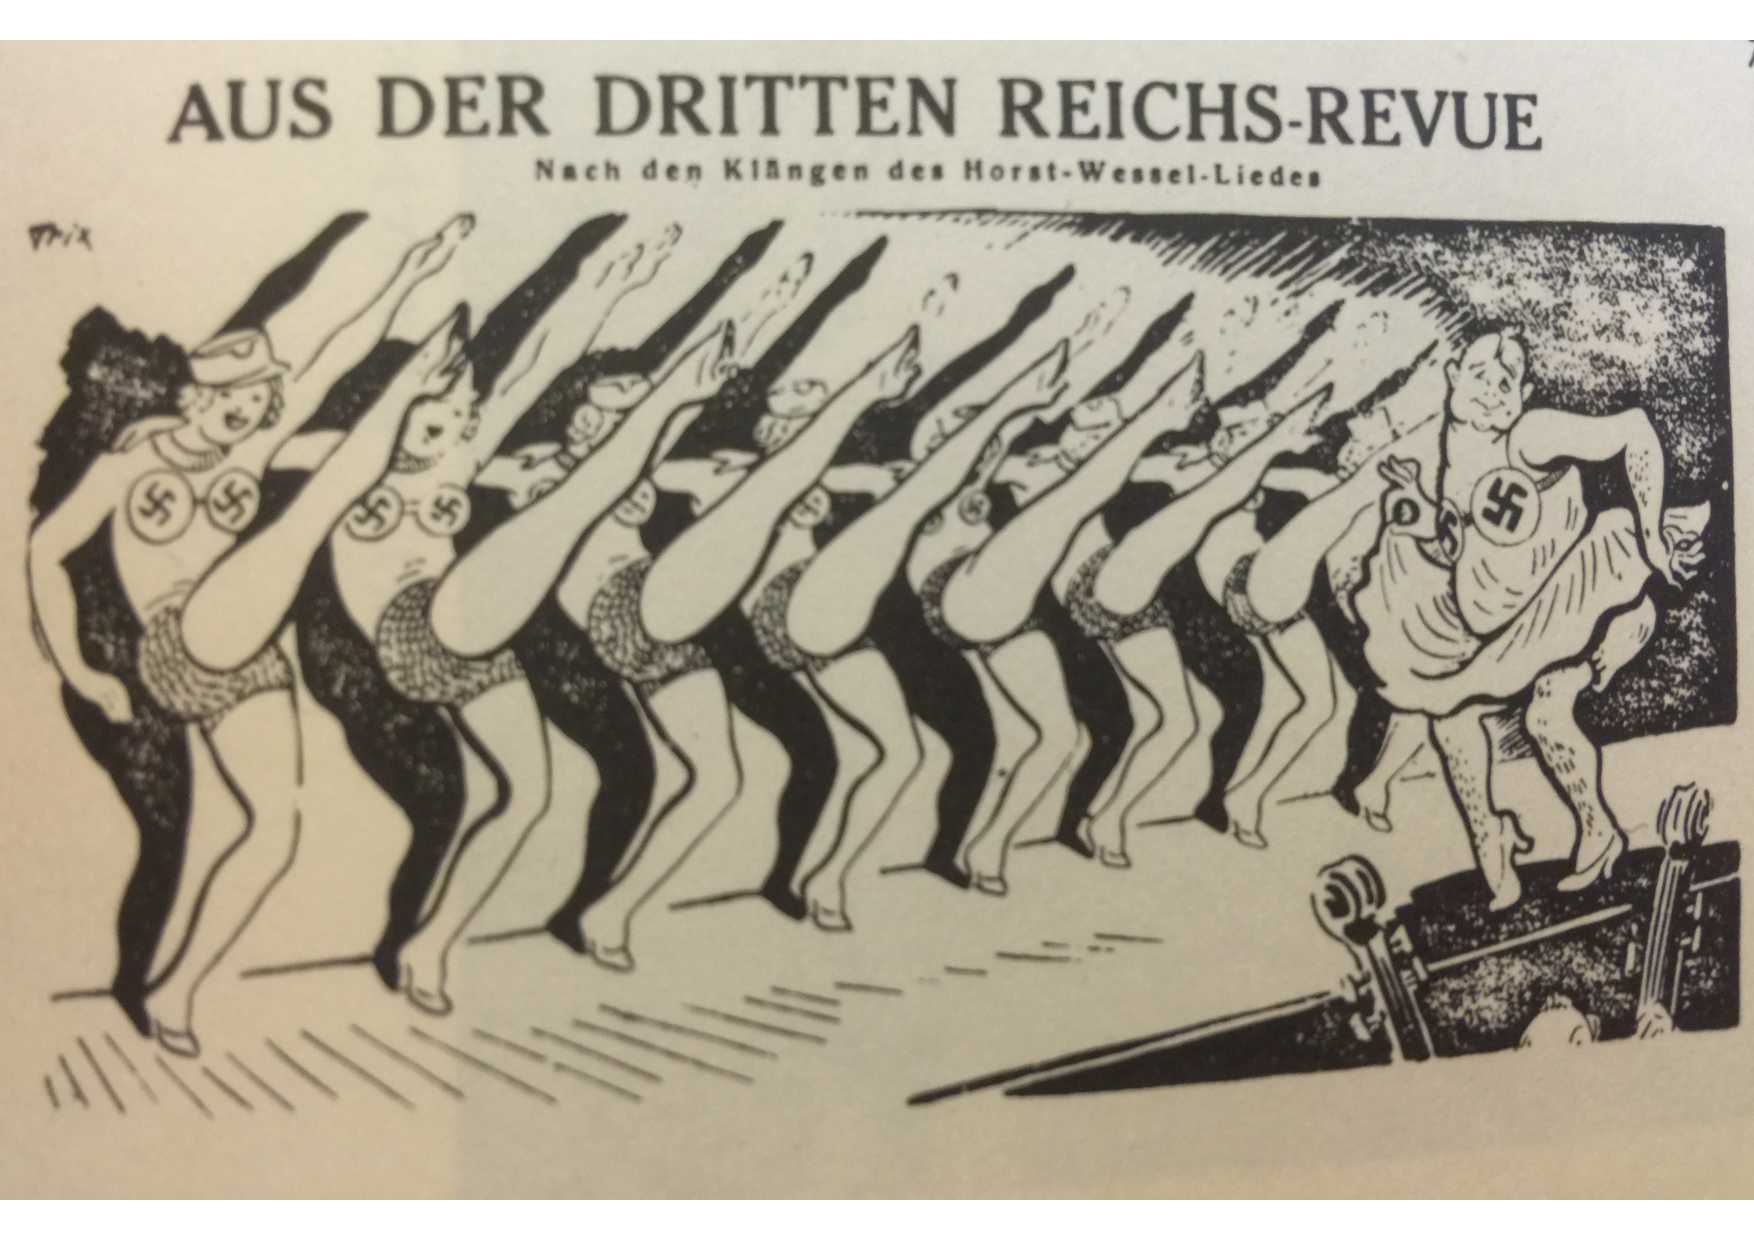
\includegraphics[width=8cm]{DrittenReichsRevue.pdf}
\caption{第三帝国のレビューより\cite{関}}
\label{fig:rrevue}
\end{center}
\end{figure}

ここで茶化されているのは突撃隊幕僚長のレーム(R\"ohm)です. 彼はナチス
(NSDAP)の古参党員の一人で, その上, ヒトラー(Hitler)の古くからの友人でした.
 ところが彼は乱暴者で生粋の男色家として著名で, 「\textbf{私のところにいる男
 たちは法律に反した特別な事に慣れねばならない}」と豪語し, 彼が在任中の突撃隊
で同性愛が横行したといいます. さらに彼は「国家社会主義」の「社会主義」に重点
を置いて「第二革命」を主張し, 突撃隊の国軍化を図ったことから国防軍に警戒され,
最終的に親衛隊によって所謂「長いナイフの夜」で粛清されてしまいます. この粛清
でナチス左派が大量に粛清され, 粛清以降は同性愛は徹底的に禁じられることになり
ます\footnote{「ドイツ第三帝国」\cite{クラーザー}が文化的な側面にも言及があり
良い本です.また, ジョークについては「ヒトラー・ジョーク」\cite{関}が決定的で
しょう. この本からヴィスコンティ(Visconti)の「地獄に堕ちた勇者ども(The Damned)」
が連想される図\ref{fig:rrevue}を選びました.}
\newpage

\begin{wrapfigure}{l}{5cm}
\includegraphics[width=6cm]{Breker2_relief.pdf}
\caption{ブレーカー:戦士の出発}
\label{fig:breker1}
\end{wrapfigure}

ここでナチス公認芸術は図\ref{fig:breker2}のような英雄的なものに
加え, 図\ref{fig:breker1}のように何だかよく判らないけどカッコエー代物
(裸体にマントがス・テ・キ$\heartsuit$)だとか, まあ随分と同性愛一歩手前の
際疾いものだったのです\footnote{女性絵画になると... ちなみに女性画の公認
巨匠ツィーグラー(Ziegler)は「\textbf{ドイツ恥毛の巨匠}」と呼ばれていたそう
です. 苦言を呈する党員も居たそうですが「\textbf{兵士達は美しいものに飢えて
いるんだ!}」の一言で片付けられたとか.}. こういった代物に, その胡散臭さは
さておき男の私でも「憧憬」を感じてしまうのです. 実際, こういった偉丈夫に
「\textbf{俺に付いて来い!}」と壁ドンされるとどうですか? 「\textbf{うほ!?}」
とならないにせよ「\textbf{面白い冒険が始まりそう..}」と思ってフラフラと
付いて行く男も多いのではないでしょうか? ただ, 古代ギリシャの同性愛は性的な
もの以上に「\textbf{若者は年長者の名声と知恵に憧れ, 年長者は若者の若さと
美に憧れる}」という至って素朴なものだったのではないかと私は思っています.
\newline

なお, ナチスはギリシャ文明を北方化したくて仕方なかったようです.
 実際, 歴史的にも北方からドーリア人(\textgreek{Dwrie'is})等の侵入がミケーネ
文明崩壊の原因の一つとされ, スパルタ(\textgreek{Spart'a})は先住民を征服して
とんでもない占領政策を続けているのでそう言いたくなるのも判らない訳でもあり
ません. これもゲーテ(G\"othe)が悲劇ファウスト(Faust)\cite{ゲーテ}で,
 本来の人形劇のファウストで絶世の美人の例でしかなかったヘレネー
(\textgreek{<El'enh})をヘレニズム文明そのものとし, それをドイツ・バロック的
なファウストと結婚させることで自らの古典主義を賛美したあたりからでしょか
\footnote{ヘレネー:「私はひどく遠くにいるような, そのくせ近くにいるような
気がします..」\cite{ゲーテ}第二部,第三幕}?  ゲーテはさておきその亜流連中に
とってはフランスがラテン文化の後継者なら, ドイツはより源流のギリシャ文明を
取るといった安易な民族主義が根幹にあったのかもしれません. なお, 野蛮な
ゲルマニアをそのまま受け入れるようになったのはロマン主義も後期に入ってから
のことです\footnote{当時のお隣のロシア帝国も同様で, 19世紀のチャイコフスキー({\cyr{Cha{\u i}kovski{\u i}}})のバレエは主に中世ドイツの宮廷やフランス的
な貴族の館の話ですが, 20世紀初頭のプロコフィエフ({\cyr{Prokof{\cprime}ev}})
やストラビンスキー({\cyr{Stravinski{\u i}}})になるとスキタイ人や古代ロシア人,
 でなければ民話といったあんばいです. では日本は? 政治的風潮で軍国主義を高貴と
讃え, 米英を卑しい商人の国と軽蔑したのが第一次世界大戦中のドイツ\cite{クラウス},
 日本ではそれを1930年代後半と20年近く遅れています.}.
\newline

ともあれナチスについて言えば, 19世紀末の夜郎自大的な民族主義にどっぷり染まり,
 ワーグナー(Wagner)のオペラの絢爛豪華さに感激した「\textbf{永遠の半端者}」,
 要するに2ちゃん用語の「\textbf{厨房共}」で, 「\textbf{聖なる愚か者}」の
Siegfriedを「\textbf{金髪の野蛮人}」に単純化して捉え, それで彼等の青少年を
染め上げた結果, のちにギリシャ文明の担い手になったドーリア人どころか
西ローマ帝国を崩壊させて暗黒時代を招来したヴァンダル族(Vandal)以上の想像を
絶する惨禍を招いてしまったのです. 19世紀初頭のドイツはヘルダーリン
(H\"olderlin)によれば「\textbf{人がいるが人間がいない!ドイツ人ほど支離滅裂な
国民はいない. 職人はいる, だが人間がいない. 思想家はいる,だが人間がいない.
 牧師はいる, だが人間がいない.}」と嘆く有様で,  この状況はのちの哲学者
 ニーチェ(Nietzsche)も同意し, 「ツァラトゥストラはこう言った」で
 「\textbf{耳が肥大化した人間}」等の戯画化で「\textbf{専門バカ}」や
「\textbf{教養主義の俗物}」を茶化しているのです(\cite{ツァラトゥストラ},
救済)\footnote{ヘルダーリンのそれは「ヒューペリオン」にて失意の主人公が
ドイツに行ったときの感想です. ニーチェがそれを受けていることはその有様を
「\textbf{戦場か屠殺場のように}」とヒューペリオンと同じ表現になっている
ことで判ります.}.
\newline

さて, ニーチェの著作「悲劇の誕生」\cite{悲劇の誕生}を読むと猛烈な古代
ギリシャへの憧れが見受けられます. この「悲劇の誕生」ではいわゆる
「ディオニューソス(\textgreek{Di'onusos})」的なるもの, つまり情念と
「アポローン(\textgreek{>Ap'ollwn})」的なるもの, つまり理念の対峙という
ことをはじめて主張した論文で, 同時にワーグナーの悲劇をよいしょするもので
あったために「\textbf{未来の文献学}」\footnote{ニーチェの本来の専門は文献学
で, ワーグナーは自分の音楽のことを「\textbf{未来の音楽}」と呼んでいたこと
への当て付けです.}とまで皮肉られる結果になっています. その結びの一節に
「\textbf{美がこのように絶えず押し寄せてくる時...}」とありますが, 実に古代
ギリシャは偉大なのです. ところが我々日本人は非常に残念なことに文明開化の
時点で目覚しく発展しつつあるプロシア=ドイツ帝国に目を奪われ, その結果,
 ドイツ好きは沢山居ても, 西洋文明の源泉たるギリシャへの関心が斯くも少ない
のが現状なのです\footnote{文学では「潮騒」の三島由紀夫でしょうか.}.
\newline

そしてこの駄文の目標はギリシャ哲学と計算機科学を強引に結び付けようと
する分不相応な企てなのです. 時代を越えてファウストがヘレナに憧れ, 彼女と
共にあらんとするように私もそれを目指すのです. 

\section{プラトンのイデア論}


さて主題の「\textbf{オブジェクト指向プログラミング(Object Oriented
 Programing)}」ですが, これはオブジェクトという概念を導入することで
プログラミングの生産性向上を図っているものと説明されます. 具体的にはクラス
というオブジェクトの雛形が用意され, その雛形を使ってプログラムが扱うデータ
に対応するインスタンスを生成して処理を行うこと. そして, クラスは属性や
メソッドをあらかじめ備えているので, そのインスタンスの処理でそれらが使える
こととクラスには親子関係に類似した階層構造があり, 属性やメソッドが継承と
呼ばれる手法で下位のクラスのインスタンスでも使えるという長所があることで
しょうか.
\newline


このオブジェクトがクラスから創られる様子を説明するためにプラトン
(\textgreek{Pl'atwn}, Plato)の「\textbf{イデア論(Theory of Forms)}」が引っ
張り出されることがあります. まず, プラトンのイデア論によれば我々が考察の
対象とする現世の「\textbf{個体(individual)}」に対しては
「\textbf{思惟によってのみ知られる世界}」, すなわち「\textbf{イデア界}」に
「\textbf{イデア(\textgreek{>id'ea}, idea)}」が存在し, 個体はそのイデアの
像であるというものです. だから貴方のそばに居る三毛猫の「\textbf{みけ}」には
対応する「\textbf{三毛猫のイデア}」が「\textbf{イデア界}」に存在し, その
イデアを現世に投影したものが貴方のそばに居る「\textbf{みけ}」であるという
主張です. なお, プラトンのイデアは思惟によってのみ知覚できることに加え,
 さらには「\textbf{永遠不滅}」といった超越的な性質を持っています. このこと
からイデアは現実にある対象を「\textbf{理想化したもの}」で, ちょうど
「\textbf{鋳型}」のような役割をしていると言えるでしょう. ただし, プラトン
はイデア界こそが真実の世界で, 現世はイデアが投影された影の世界, 要するに
模造品の世界と見なしています(c.f. 「洞窟の比喩」\cite{国家}).
\newline


ところでオブジェクトが計算機上のデータとして「\textbf{実体化}」する
ことを「\textbf{インスタンス化(instantiation)}」, それから
「\textbf{実体化したオブジェクト}」のことを
「\textbf{インスタンス(instance)}」と呼びますが, 
「\textbf{イデアの現世における実体化}」も英語では同じ
「\textbf{instantiation}」になります. と, このようにクラスとインスタンスの
関係は前述のイデアと実物との関係に類似しています. ところでイデアを誰が実体化
し, どのような理由で実体化したのかという素朴な疑問になると途端にプラトンは
歯切れが悪くなります. まず誰がイデアを実体化させたのかと言えば,
 「\textbf{デーミウールゴス(\textgreek{dhmiourg'os})}」がイデアを模倣して
世界を創世し, その模倣の理由は貧欲な神「\textbf{エロース(\textgreek{>'Erws})}」
がイデアの美に憧れたからと述べていますが納得できるものではありません.
 また, イデアは美や善に関わるもので醜いものや悪にイデアは存在しないと
述べていますが, 「\textbf{何が美なのかをヒキガエルに聞いてみろ!}」と
ヴォルテール(Voltaire)ならずとも言いたくもなるでしょう.
\newline


このような「\textbf{機械仕掛けの神(Deus ex machina)}」\footnote{
古代ギリシャ悲劇で収拾がつかなくなった話を解決するためにいきなり舞台に神
を登場させること(たとえばソフォクレース(\textgreek{Sofokl'hs})の悲劇
「ピロクテーテース(\textgreek{Filokt'hths})」の終盤に現われるヘーラクレース
(\textgreek{<Hraklns}))がありましたが, その都合の良さに対する皮肉です.}を
持ち出されても信じるしかないところは哲学というよりも宗教です. 実際, のちの
ヘレニズム文明では, プラトンのイデア論を基に超越的な
「\textbf{一者(\textgreek{to >'en}, to hen)}」とその一者からの流出による
世界の創造(流出説)を取り入れた「\textbf{新プラトン主義}」\footnote{
「新プラトン主義」とは後世の呼び名で, その信奉者達はプラトンの考えに合致
するものと思っていました.}, デーミウールゴスによる悪しき世界の創造, 星辰の
支配を受けて肉体という牢獄に囚われた人間, そして死後の超越的な神への帰一を
柱とする「\textbf{グノーシス主義(\textgreek{Gnwsis})}」\footnote{中近東では
未だに少数派としてちらほら残っているようです.}へと繋がります.
\newline


\begin{wrapfigure}{l}{4cm}
\includegraphics[width=4cm]{HermesTrismegistusCauc.pdf}
\caption{ヘルメス・トリスメギストス}
\label{fig:trismegistus}
\end{wrapfigure}

このグノーシス主義の文献に「\textbf{ヘルメス文書}」と呼ばれる一群の文書が
あります. これはヘルメス・トリスメギストス(三重に偉大なヘルメス, Hermes
 Trismegistus, \textgreek{<Erm\~es Trism'egistos})が記したとされたものです.
 ここでのヘルメスはギリシャ神話の神ヘルメスとエジプト神話の神トートが
ヘレニズム時代に融合したもので, 錬金術では「\textbf{賢者の石}」\footnote{
賢者の石は錬金術師が探し求めた究極の霊薬で, 鉄などの非貴金属を貴金属の金に
変え, 人間を不老不死にするものです.}を実際に手にした人物\footnote{
図\ref{fig:trismegistus}の恰好の人物どこかで見たことありませんか?
 MITのSICP(Structure and Interpretation of Computer Programs)の扉絵の人物に
似てますね. つまり$\lambda$ - 函数概念 - は計算機科学の「\textbf{賢者の石}」
で「\textbf{$A$ にして $\Omega$}」なのです!
Sanctus, sanctus, sanctus, dominus deus sabaoth.}とされています\cite{錬金術}.
\newline 


そのヘルメス文書の一つの「ポイマンドレース(Poimandres)」\cite{柴田}によると
人間は元来, 神の子で美しい神の似姿として創られたとされます. 彼があるとき高次
で純粋な天上界からより下位の地上に向うことで星辰の支配を受けることになり,
 最後に地上にてフュシス(\textgreek{f'usis}, 自然)内に写った自分の姿に恋する
ことでフュシスと愛欲に陥いり「\textbf{フュシスは愛する者を捕へ, 全身で抱き
しめて互に交わった}」その結果, 人間はフュシスに捕えられてしまったといいます.
 この伝説\footnote{おおよそ宗教, あるいは宗教的な代物はその伝説を続々と生成
するものです. 現在でもカトリックでは列聖で伝説が生成され, 共産主義はその英雄
を量産するといった有様です. }が人間の本質が神の似姿のために不死であるものの
消滅する肉体に囚われ, その上, 星辰に支配された存在\footnote{星辰に支配される
からこそ占星術に意味があるのです.}であるという二面性を持つことへの説明に
なっています. この伝説にはヘレニズム文化圏でオリエント諸国の占星術の影響と
イデア論を中核に哲学が宗教へと変じて行く様子が刻印されているとも言えるでしょう.
\newline

この世はデーミウールゴスが誤って創造したものだという厭世的な観点は新プラトン
主義はもちろんのこと, キリスト教徒の主流派からも反駁されます\footnote{全知
全能の神が半端なことをする筈がないという反論です.}. それどころか本質的に
黙示的な宗教であったキリスト教は新プラトン主義の影響により徐々に合理的な
宗教へと変貌します. この変化は初期のキリスト教哲学にて教父と呼ばれる神学者
によるもので, 特に若い時分にマニ教徒\footnote{マニ教はグノーシス主義の宗教の
中では最も勢力を奮った世界宗教でした. 近年, 日本でもマニ教の曼荼羅絵が発見
されている程です.}でもあった教父アウグスティヌス(Augustinus Hipponensis,
 Augustine of Hippo)を通じて, 新プラトン主義が初期のキリスト教の理論付けに
用いられます. その際に新プラトン主義のフィルターを介した形でアリストテレス
(\textgreek{>Aristot'elhs}, Aristotle)の哲学も部分的に導入します
\footnote{ともすればプラトンに批判的なアリストテレスの哲学が本格的に
導入されるのは12世紀以降の話です\cite{アリストテレス1}\cite{普遍論争}.}.
 キリスト教と古代の間には大きな断絶があるのも事実ですが, ヘレニズム文明の
宇宙観, 星辰信仰やイシス信仰をマリア崇敬として引継ぐ等, ヘレニズム文明を
色々と引き継いでいる一面もあるのです.
\newline

ここで本題に話を戻しますが, プラトンのイデア論はオブジェクト指向
プログラミングのクラスとインスタンスの関係に類似がみられるものの,
 インスタンス化の類似に留まります. 実際, 真っ新なシステムで「三毛猫!」と
唱えれば完全無欠の三毛猫のクラスが降臨することもなければ, 我々が扱おうと
するオブジェクトの雛形たるクラスは天与のもの, すなわち
「\textbf{神聖ニシテ侵スヘキアラス}」な代物ではなくて現実のオブジェクト
からクラスを抽出しなければならない, つまり我々が扱う対象は
「\textbf{どのようなものであるかを語れる}」もので, クラスは
「\textbf{何であるかを語るもの}」でなければなりません. このような
ものには「\textbf{概念}」があります. そこで概念というものが何であるかを
述べることにしましょう.

\section{概念について}


「\textbf{概念(concept)}」はイデアのような超越的なものではありません. 概念が
実在するかどうかは中世以来の論争\cite{普遍論争}になっていますが, その存在の
有無はさておいて, 概念は我々の対象に対する理解に従うものです. 実際, この概念
がどのようにして得られるかと言えば, 対象を特徴付ける「\textbf{徴表}」,
 つまり「\textbf{属性}」を抽出し,これらの属性を共通性で纏めることで得られます.
 要するに「\textbf{何であるか?}」や「\textbf{それがどのようなものであるか?}」
という問に対する回答から, それを特徴付ける形や色や機能といったものを纏める
ことで得られるものなのです. このように我々が対象を目前にしたときに
「\textbf{それをどのように語るか}」ということこそが本質です. そして概念は人間が
認知し得る具体的なもの, たとえば対象の形や色といった
「\textbf{形相(\textgreek{>e'idos})}」から出発し, 我々が対象をどのように語るか
ということ, つまり「\textbf{説明規定(\textgreek{l'ogos}, ロゴス, account)}」
なのです.このように概念はイデアとは逆に具体性から抽象性・普遍性を目指すもの
です. なお, 概念は「\textbf{名辞(term)}」して現れますが, 名辞はあくまでも概念
が乗る器であって概念そのものではありません.
\newline

\begin{wrapfigure}{l}{4.5cm}
\includegraphics[width=4.5cm]{Plato_and_Aristotle_in_The_School_of_Athens,_by_italian_Rafael.pdf}
\caption{アテナイの学堂より:プラトンとアリストテレス}
\label{fig:Plato-Aristotle}
\end{wrapfigure}


そして「\textbf{それが何であるか?}」や「\textbf{それがどのようなものであるか?}」
といった問に対する回答についてより深く考察した人物がアリストテレスです.
 このアリストテレスとプラトンの思索の方向性の違いはラファエロ(Raffaello)
の有名な絵画「アテナイの学堂」\cite{アテナイ}にて中央に起立している両者の手の
違いで表現されていることはよく知られていることです. 図\ref{fig:Plato-Aristotle}
に示すようにプラトンは天上(イデア=抽象)を指し, アリストテレスは地上(形相=具象)
を示すという風にです\footnote{ルネサンス期において新プラトン主義は非常に大きな
影響を与えています.}. つまり, イデアは地上の個体から超越した存在であるのに対し,
 概念は個体の徴表から取り出されるものだということなのです.
\newline

さて, そうして得られた概念は「\textbf{AはBである}」という命題であれば,
 複数の主語(A)の述語(B)となり得るという性質を持ちます. つまり, 概念はある
ものを語るものであり, だから対象Aを語るときに「AはXだ」となれば, まず概念
は対象Aの述語Xとして現れます. さらに対象Aだけに限定されずにほかの対象Bに
ついてもXであると言える可能性があるのです. この複数の主語に対して述語になる
性質を「\textbf{普遍}」と呼びます\footnote{いろいろなものを取り替えて使える
ものに「ユニバーサル」の名前を冠したものがあるのは, この主語を取り替えられる
性質に擬したためです.}. たとえば「\textbf{猫}」という「\textbf{概念}」は,
 その辺にいる「みけ」や「たま」, その他の貴方の周囲の野良猫 $x$ からでも
「\textbf{$x$ は猫である}」という命題が作られます. だから「\textbf{猫}」と
いう「\textbf{概念}」は\textbf{普遍}なのです. その一方で「みけ」や「たま」
は個体に強く結びつけられて「これがたまです」という命題のように個体を特定する
もので普遍ではありません. 
\newline

次に「猫」という括り(あつまり)に対して「三毛猫」, 「黒猫」, 「白猫」,
 「虎猫」等の毛並で分類することもできます. これらは「猫」の毛並について
述べたもので, こちらは「猫」という概念よりも個々の猫をより詳細に説明する
ものになっています. 逆に「猫」は「三毛猫」等を包括して説明しようとするもの
になっています. このように概念には「\textbf{類似する個体をまとめてより
包括的に説明しようとする概念}」, すなわち「\textbf{個体から離れた側の概念}」,
 それから逆に「\textbf{個体をより詳しく説明しようとする概念}」, 
 すなわち「\textbf{個体に近い側の概念}」の二つがあることが判ります. そして
「\textbf{対象を類似する対象とまとめて包括的に語ろうとする概念}」は
「\textbf{個体をより詳しく説明する概念}」を包含します. このように一つの
対象を語る二つの概念があって, 一方の概念が他方の概念を包含するときに包含
する側の概念のことを「\textbf{上位概念}」と呼び, 逆に個体をより詳しく
語ろうとする概念のことを「\textbf{下位概念}」と呼びます. これらの二つの
概念を比較すると上位概念がより普遍になります. たとえば「三毛猫は猫である」
という命題では「猫」が上位概念, より細かく個体の「みけ」を説明している概念
が下位概念の「三毛猫」になります. 実際, 「三毛猫」は「猫である」と
「毛の色が黒・茶・白の三色である」の二つの性質が述べられるからです. また,
 「三毛猫」よりも上位の概念である「猫」が「三毛猫」よりも大雑把な説明である
ことも判るでしょう. しかし, 大雑把であるがゆえに「猫」という概念には
「白猫」, 「黒猫」, 「虎猫」といった「三毛猫」以外の概念も包含されて
「三毛猫」よりも「猫」がより包括的, すなわち, より普遍であることも理解される
でしょう. 
\newline

また上位概念のことを「\textbf{類概念}」, あるいは
「\textbf{類(genus)}」, 下位の概念のことを「\textbf{種概念}」 あるいは
「\textbf{種(species)}」とも呼びます\footnote{類と種の関係をここでは上位概念
と下位概念として述べていますが, 「\textbf{種類}」という言葉があるように
類(genus)と種(species)は分類学で属(genus)と種(species)に対応し, 属の直下に
種があってもその間には何かが入ることはありません. このように種は類の直下に
ある概念としての性格がありますが, ここではそのような限定はしていません.}.
 先程の「猫」で解説するならば「三毛猫の類概念」が「猫」, 「三毛猫」が
「猫の種概念」になります. そして「\textbf{種}」の違いを示す徴表(特徴)を
「\textbf{種差}」と呼びます. たとえば先程の「三毛猫」, [虎猫」, ... の例
では「毛並」の違いが種差になっています.それから「上位」とか「下位」では
どちらがより普遍的であるかということに対応し, 具体的には普遍的な概念の外延
は下位概念の外延よりも広くなります. つまり, 概念の外延の包含関係にも対応
するのです. そしてには概念にはその上限と下限があります. ここで最上位の
上位概念のことを「\textbf{範疇(カテゴリー, Category)}」, 最下位の下位概念を
「\textbf{単独概念}」, あるいは「\textbf{個体概念}」と呼びます. この個体概念
は個体を直接指示する概念であり, 当然, 個体に最も近い概念になります. それに
対して範疇は個体を含む概念の中で最も普遍的な概念となります\footnote{だから
メニュー等では最上段が「\textbf{カテゴリー}」という名称で分類されているの
です.}.
\newline


この概念の階層構造についてはアリストテレスが「範疇(カテゴリー)論」等
の著作で述べています. ところで, ともすればプラトンに批判的なアリストテレス
は「新プラトン主義」の哲学者からは「師の考えを秘匿するために批判していた」
と捉えられていたようで, 彼の論理学は新プラトン主義の哲学への入門書として
重要視されます. 特に古代ローマ帝国の哲学者ポルピュリオス
(\textgreek{Porf'urios}, Porphyry of Tyre)が記述した
「\textbf{手引(エイサゴーゲー, \textgreek{E>isagwgh'},Isagoge\cite{Barnes}}」
が哲学を学ぶにあたって最初に読むべき本とされていました. この「手引」によると
「\textbf{ものごとを語る}」ということには今まで述べてきた「\textbf{類}」,
 「\textbf{種}」と「\textbf{種差}」に加えて「\textbf{特有性}」と
「\textbf{偶有性}」があると述べています. まず, 類や種は「\textbf{それが何であるか?}」という問に対する
回答です\footnote{類(genus)や種(species)という言葉の語源はギリシャ語の
\textgreek{g'enos}, \textgreek{e\t{>i}dos}に由来し, 共に「\textbf{形}」
という意味があります. このことから概念は形の類似や違いをもとに分類していた
経緯が判るでしょう. 分類学で当初はその形態, ダーウィン以降は進化, 現在はDNA
等の分析が入っています.}. それから「\textbf{種差}」と「\textbf{特有性}」と
「\textbf{偶有性}」は「\textbf{それがどのようなものであるか?}」という問に
対する答として語られるものです. まず「\textbf{種差}」については
「\textbf{種を特徴付けるもの}」, それから「\textbf{特有性}」は
「\textbf{それが何であるかを語るものではないが指摘できるようなもの}」, つまり
固有の特徴のことです. それに対して「\textbf{偶有性}」は
「\textbf{それの程度を語ることができるもの}」です. たとえば日焼けした子供の
ように「全然日焼けていない」, 「薄く日焼けしている」, 
「良く日焼けしていて真っ黒」のようにその程度が表現可能なものであり, そうで
ない状況(「日焼けしていない」)」が考えられる特徴のことです. なお, この
ポルピュリオスの「\textbf{類}」,「\textbf{種}」, 「\textbf{種差}」,
「\textbf{特有性}」と「\textbf{偶有性}」による述語の分類は非常に大きな影響
をさまざまな分野に与えています. たとえば
「\textbf{ポルピュリオスの樹(Arbor Porphyrianae)}」というものがあります:


\begin{itembox}[c]{\textbf{ポルピュリオスの樹}}
{\tiny
\begin{tikzpicture}
\Tree [.本質的存在 [.物体 [.生命がある [.理性的 [.人間 [.ソクラテス ]
                                                       [.プラトン ]
                                                       [.特定の人々 ] ] ]
                                       [.非理性的 ] ]
                          [.生命がない ] ]
                   [.非物体 ] ]
\end{tikzpicture}
}
\end{itembox}

これは本位概念の類を下位概念の種で分類することをのちの註釈者が視覚化した
もので, 様々な分野で用いられています.
\newline

またリンネ(Carl von Linn\'e)が始めた動植物の学名の命名方法は
「\textbf{二名法}」と呼ばれますが, この方法は種による類の分類そのものです.
 つまりこの命名方法は動物/植物が属する種とその種を包含する属に対して最初に
属(genus)のラテン語での名前, それから種(species)のラテン語の名前を列記する
というものです\footnote{正に「\textbf{種類}」になっているのです.}. たとえば
人類の学名は`Homo sapiens'ですが, 属がHomoで種がsapiensなのです.
\newline

この二名法はオブジェクト指向プログラミングでも, クラスの属性やメソッド,
あるいはクラスとその直下のサブクラスの表記でも用いられています. このことから
判るように, オブジェクト指向プログラミングでは単に雛形としてクラスを準備する
ということがプログラミングの本質ではなく, 我々が対処しなければならない対象を
語り, 明確に定義付けや特徴付けといった分析を行うことこそが最も本質的なのです.
\newline


さて「\textbf{それが何であるか?}」という問いに対し, 我々はそれが
どのようなものであるかを説明するか, そうでもなければ個体を列挙して説明
するかどちらかになるでしょう. このように概念の表現には二通りの表現, 一つは
「\textbf{内包}」, もう一つが「\textbf{外延}」があります. 最初の
「\textbf{内包}」は概念が持つ徴表/属性で構成され,「\textbf{外延}」は概念が
適用される対象を列記することで構成されます. 「\textbf{猫}」という概念なら,
 その内包は「\textbf{動物である}」, 「\textbf{4本足で歩く}」,
 「\textbf{柔らかい肉球を持つ}」, 「\textbf{ニャオと鳴く}」等の属性から
構成されるでしょう. 一方で外延なら単純に「ペルシャ猫」, 「シャム猫」と
いった猫の種, 「黒猫」, 「白猫」, 「虎猫」, 「三毛猫」といった毛並で分類
する方法, あるいは「粟根さんのペットのタマ」のように個体を列記する方法に
なるでしょう. このように内包は概念を説明する述語から, 外延は概念に対応する
具体的な個体や下位の概念の列記で構成されます.
\newline


そして内包と外延には「\textbf{内包外延反比例増減の法則}」と呼ばれる
関係があります. つまり, 内包が増大するに従って外延が減少し, 外延が増加すれ
ば内包が減少するという反比例関係です. たとえば「猫」という概念に対して
「茶、黒、白の三色の毛並である」という内包を追加すると「三毛猫」以外の
「白猫」, 「黒猫」等の猫が「猫」と「茶、黒、白の三色の毛並」の外延から消え
てしまいます. 逆に「三毛猫」という外延に「白猫」という外延を追加すると
「茶、黒、白の三色の毛並である」という内包が消えてしまいます. このように内包
が増えるということは, それだけ述語付けられることで個体に近付くために外延が
絞られ, 逆に外延を構成する個体が増えれば個体から離れて普遍的な事柄を抽出
することになるために内包が減少するということなのです. 
\newline

なお外延で表現された概念は内包で規定することができますが, 逆に内包で
規定された概念は外延で表現できるとは限りません. それに加えて任意の命題が
外延を持つとは限りません. たとえば `$x \neq x$' という命題の外延は存在しま
せん. この命題は「\textbf{ラッセルの逆理}」と呼ばれる非常に有名な逆理です.
 この非常に単純な命題をラッセル(Russell)自身がより分かり易くしたものが次に
述べる「\textbf{床屋の逆理}」です:

\begin{itembox}[c]{{床屋の逆理}}
\quad とある村には床屋が一軒あります. その床屋の主人は自分で髭を剃らない
人の髭だけを剃ると言っています. では, その床屋の主人の髭は誰が剃ればよい
のでしょうか?
\end{itembox}

この逆理の本質は前述の `$x \notin x$' という命題で, 
「\textbf{自分自身を元として持たないもの}」と自己を引用するという循環的
な定義方法を採用しています. そして, この逆理のためにフレーゲ(Frege)の
論理主義\footnote{数学を論理学から導出しようとする立場です. 初期は
フレーゲの「算術の基本法則」\cite{フレーゲ}, 後期はラッセルの
「Principia Mathematica」\cite{Russell}が有名です.}は破綻してしまいます.
\newline


ポアンカレ(Poincar\'e)は「科学と方法」\cite{ポアンカレ}にて幾つかの
逆理を分析し, 循環論法を含む定義に問題があると述べています
(\cite{ポアンカレ},p.204). たとえば「偶数の集合」や「身長170cm以下の人の集合」
といった集合の定義では「自然数の集合」や「人間の集合」といった根本の概念に
触れずに集合が定義ができており, このような定義方法を「\textbf{可述的}」と
呼びます. そして, 床屋の逆理のように循環論法に訴えなければ自分自身を定義
できない定義方法を「\textbf{非可述的}と呼び, この非可述的な定義に問題が
あると述べています. そこでラッセルは逆理を排除するために「\textbf{型理論}」
と「\textbf{悪循環原理}」を公理系に導入し, それで非可述的な命題を排除した
ものの, 今度は数学的帰納法が使えないという副作用が生じてしまいました.
 この事態は非常に厄介で, この難点を除外するために「\textbf{還元公理}」と
呼ばれる公理を導入すると今度は天下り的な性格が問題になるといった有様で,
 これらの試みが成功したとは言えません\cite{Russell}. なお, 現在の集合論
では後述の集合の公理系で「\textbf{集合}」を定め, それ以外の命題の外延の
ことを「\textbf{類}」, あるいは「\textbf{クラス}」と呼んで集合と区分し,
 集合の公理系によって「ラッセルの逆理」自体を排除しています.

\section{定義付けること}

さて我々は事物を抽象することで概念に辿りつきました. 逆に
「\textbf{Xを充すものがYである}」とも言える筈です. この操作を
「\textbf{定義付ける}」と言います. そして「\textbf{定義付ける}」ということに
「\textbf{タマは猫である}」 のように類や種で定義付ける「\textbf{実体的定義}」,
 あるいは 「\textbf{分析的定義}」と呼ばれる方法と
「\textbf{点は平面上の平行でない二直線の交わりとして構成される}」という点の
定義のように対象がどのような条件で発生, あるいは成立するかを記述する
「\textbf{発生的定義}」, または 「\textbf{綜合的定義}」と呼ばれる内包的な
定義があり, それと外延的な定義として
「\textbf{実例, または代表・典型を用いた定義}」があります.ちなみに
アリストテレスが創始者である逍遥学派の「\textbf{定義}」は類と種や種差を
用いてその「\textbf{説明規定}」を与えることです.


\section{プラトニズム}


では概念やイデアは実在するものでしょうか? イデア論を認めるのであれば,
 イデアは個体とは別個に存在しなければなりません, ところが概念の存在はなか
なか厄介な問題です. たとえば「三毛猫のみけ」を観察することで「猫」や
「三毛猫」といった概念に到達できるとはいえ, だからといって「みけ」が「猫」
や「三毛猫」といった概念に先立って存在している訳ではありません. それ以前に
存在した猫や三毛猫によって「猫」や「三毛猫」が定義されているからです.
 アリストテレスは範疇論にて類や種を第二の本質的な存在と呼んでいますが,
 それらが実際に存在するものかどうかを明確に述べていません. また前述の
エイサゴーケでも著者のポルピュリオスが類や種といった概念(普遍)が存在する
ものであるかどうかを触れないと最初の章で述べており, エイサゴーゲをラテン語に
翻訳したボエティウス(Boethius)による第二注釈が西洋の中世スコラ哲学の
「\textbf{普遍論争}」を引き起すことになります\cite{普遍論争}.
\newline


ここで物理学の原理や数学の定理の方が先に存在して, それらを人間が発見する
と考えるか, 到達した概念から原理や定理が導出されるものなのかといった議論にも,
 この議論は繋がります\footnote{「\textbf{発見}」なのか「\textbf{発明}」なのか?}.
 ここで事物の前に概念があると考える立場を「\textbf{プラトニズム(Platonism)}」,
 あるいはプラトンの「\textbf{実在論(realism)}」と呼びます. それに対して事物の
あとに概念があると考える立場を「\textbf{唯名論(Nominalism}」と呼びます.
\newline


このように実在が問題となった背景ですが, アリストテレスが創始し, そこから発展
した論理学, すなわち伝統的論理学で扱う命題には
「\textbf{存在含意(external import)}」と呼ばれる条件, つまり, 命題の主語が
存在しているという暗黙の条件があります. これは古代ギリシア語が属する印欧語族
にて `A = B' という命題の主語Aと述語Bの関係を表現する「\textbf{繋辞(copula)}」
に「\textbf{存在動詞}」が用いられていることが関係しています. たとえば日本語
の「AはBである」\footnote{「AはBで\underline{ある}」という命題に
「\textbf{ある}」が何気に含まれていることに, このような用語を作り定着させた
明治の人々の何気ない凄さを私は感じます.}を印欧語族の一つである英語で
「A is B」と置換した場合, 日本語の「は」はAとBが一致すること意味する以上の
意味を持ちませんが, be動詞は主語のAが存在するという意味が付随する存在動詞
であるために「Aが存在して A = B である」の意味を持つ命題として捉えることが
できるのです. ただし, 現代の論理学に存在含意はありません.
\newline 

また伝統的論理学は主語と述語の関係の考察を行なう「\textbf{名辞論理学}」
であり, それに対して現在の論理学は命題を考察するために「\textbf{命題論理学}」
と呼ばれます\footnote{伝統的論理学に決定的に欠けているのが「\textbf{すべて}」
や「\textbf{存在する}」に対応する量化詞です.}. さて, 伝統的論理学の命題は,
 その主語に対して存在含意を前提にして論理学が構築されているために
「\textbf{非存在}」のものや「\textbf{仮説}」に対しては三段論法等の推論が行え
ないことになります. しかし, ここでイデアや概念といった普遍の存在を認めて
しまえば, 自動的に存在含意を充して推論を行う際の障害がなくなるのです.
とはいえイデアにはその超越性から色々と面倒な問題が生じます.
\newline

最も有名なイデア論に対する反論が「\textbf{第三の人間}」と呼ばれ, 
 これはイデア論者の主張するようにイデアの存在を認めると「\textbf{人間自体}」
という人間の類としてのイデアに加えて「\textbf{ソクラテス}」や
「\textbf{プラトン}」といった個人のイデアがあります. するとこれらのイデアで
人間として類似していることを示す尺度として, これらとはまた別の人間のイデアが
必要になります. これを「\textbf{第三の人間}」と呼びます. この第三の人間の存在
を認めると, 次はその「\textbf{第三の人間}」と個々の人間や人間自体のイデアとの
類似の尺度になる第四のイデアが必要になり, 以降, 第五, 第六...の人間が存在する
ことになるというものです.  この有様にプラトンの弟子であったアリストテレスも
「形而上学」\cite{アリストテレス2}にて「\textbf{物を数えようとする場合に,
 数が少なくては数えられないと思って, その数を増やして数えようとする者の
ごときである}」と批判しています\cite{アリストテレス2}
\footnote{形而上学 第一巻九章}.
\newline


ものの鋳型としてイデアとして考えてこの有様ですが, 理想的な人間として
例えられるソクラテスにしても, 最初は赤ん坊で, それから子供, 若者, 壮年,
 老年といった過程を辿る訳ですが, すると, それぞれの瞬間にイデアがある筈で,
 そうすると, その瞬間瞬間のイデア同士の関係はどうなるのかと, 話が簡単に
なるどころか逆に複雑になっているありさまなのです. また種から芽が出てやがて
木になり, それが老木になって倒れて腐るといった, 個体の生成, 変化や運動,
 最後に消滅する理由がイデア論からは説明できません. 結局, 世界の生成に
しても, デーミウールゴスやエロスといったある意思を持った部外者を引っ張り
出して何とか創世神話を拵えたり, 生物の生殖の理由を説明できたとしても,
 何気ない自然現象の説明にはとても無理があるのです.


\section{形相(\textgreek{E\t{>i}dos})}

さてプラトンの弟子のアリストテレスは師匠のプラトンと異なり, 観察に
立脚した, より現実に則した考え方をしています. まず, アルストテレスの
「\textbf{\textbf{形相(\textgreek{e\t{>i}dos}, eidos)}}」はプラトンの
「\textbf{イデア(\textgreek{>idea})}」のような
「\textbf{個体から離れた存在}」(\textgreek{qorist'a})ではなく, むしろ, 現実
にある個体はこの「\textbf{形相(\textgreek{e\t{>i}dos})}」と, これといった
特性を持たない「\textbf{質料(\textgreek{<'ulh})}」との
「\textbf{結合体(\textgreek{s'unolon}}」として捉え, この形相こそがその個体
を個体たらしめる原因, つまり「\textbf{形相因}」という設計図のような働きを
するものとして捉えています. これを先程の種の話に戻すと, まず, 種に木とし
ての形相が内部に存在し, その形相が結合体としてのもう一方の質料に働きかける
ことで木として育ち, やがて形相が木から消えることで木としての特性を失って
朽ちてゆくという説明になります. このアリストテレスの考察を現在の科学と
比べてどうかと言えば, 細かな点では怪しくとも, 現代の科学も研究対象が何で
あり, どのような理由でそれがそれであるかを説明しようとするものであり, 
 この流儀はアリストテレスの考察にその源流があることが判ります. だからこそ
アリストテレスは「\textbf{万学の祖}」なのです.
\newline

さて, この形相と質料を計算機上で考えるとそれなりに面白いことが判り
ます. まず, 質料はそれ自体では何らの特性を持たないものですが, これをビット
の列に, それから形相をデータ構造等の意味付けに対応付けることができるで
しょう. すると計算機内部のデータは形相と質料の結合として表現されることに
なります. つまり, イデア論に訴えるよりも, より自然な対応付けができるのです.


\section{アリストテレスの範疇(Category)}


個体が何であり, どのようなものであるかを説明すること, すなわち,
 どのように述語付けられるかをアリストテレスは「範疇(カテゴリー)論」
\cite{アリストテレス1}にて説明しています. ここで範疇(Category)は最上位
の概念であって最も普遍的なものであると述べましたが, この哲学用語の
「\textbf{範疇}」に対応するギリシャ語のカテゴーリアー
(\textgreek{kathgori'a})は法律用語の「\textbf{責を負わせる}」という意味
のカテゴレイスタイ(\textgreek{kathgor\~{i}estai})に由来し, アリストテレス
が哲学用語として導入した経緯があります. そして, この範疇はものことを語る
ときに, ものごとに述語付けたり関連付けたりすること, すなわち, ものごとを
述定することに対応します.
\newline


アリストテレスは「範疇論」にて「\textbf{AはBである}」という命題の
述語Bが取り得るものを次の10個の範疇に分類しています\footnote{ただし,
 この分類はアリストテレスの他の著作で異なることがあるそうです.}:


\begin{itembox}[c]{{アリストテレスによる範疇}}
{\footnotesize
\begin{enumerate}
\item{まさにそれであるもの(本質的存在, 実体):「人間」,「猫」}
\item{どれだけか(量):「128cm」}
\item{どのようか(性質, 質):「面白い」, 「文法的」}
\item{何に対する(関係):「二倍」, 「半分」, 「より大きい」, 「より小さい」}
\item{どこか(場所):「千代田公園」,「ペットショップ」}
\item{何時か(時間):「昨日」, 「去年」}
\item{置かれている(態勢):「寝転んでいる」,「立っている」}
\item{持っている(所有):「靴を履いている」, 「首輪を付けている」}
\item{作用する(能動):「齧る」}
\item{作用を受ける(受動):「齧られる」}
\end{enumerate}
}
\end{itembox}


ここでの「\textbf{本質的存在(実体,\textgreek{o`us'ia})}」は
「\textbf{第二の本質的存在(第二実体)}」と呼ばれるものです. 第二があれば
第一もあり, その「\textbf{第一の本質的存在}」は「私」, 「みけ」,
「ソクラテス」等の個体で主語のみになるもの, つまり, 個体により近くて普遍性
を持たないものであるのに対し, 「\textbf{第二の本質的存在}」は「人間」,
 「猫」, 「哲学者」等の主語にも述語にもなり得るものです. そして, 類や種に
なり得るものでもあります. これらの本質的存在はギリシア語ではウーシアー
(\textgreek{o`us'ia})と呼ばれ, 英語のbe動詞に対応する「存在」を意味する
動詞\textgreek{e\~{'i}nai}を名詞化したものに由来するものです. この日本語
の訳語としては「\textbf{実体}」が当てられていますが, 本来のウーシアーの
意味する範囲は広いもので, ここでの訳語は範疇論\cite{アリストテレス1}の
新訳の用語に従っています.
\newline


なお, カント(Kant)は量, 質, 関係と様相の4綱目に分け, さらに
各自を3項目に分けて12の範疇にしています:


\begin{itembox}[c]{カントによる範疇の分類}
{\footnotesize
\begin{tabularx}{12cm}{X}
\begin{tabular}[t]{rl}
\ldelim\{{3}{30pt}[量 ]&
単一性\\
&数多性\\
&全体性\\
\end{tabular}
\\
\begin{tabular}[t]{rl}
\ldelim\{{3}{30pt}[質 ]&
実在性\\
&否定性\\
&制限性\\
\end{tabular}
%\right.
\\
\begin{tabular}[t]{rl}
\ldelim\{{3}{30pt}[関係]&
属性と実体性\\
&因果性(原因と結果)\\
&交互性\\
\end{tabular}
%\right.
\\
\begin{tabular}[t]{rl}
\ldelim\{{3}{30pt}[様相]&
可能性(不可能性)\\
&現実性(非現実性)\\
&必然性(偶然性)\\
\end{tabular}
%\right.
\\
\end{tabularx}
}
\end{itembox}


ここで重要なことは, ある物について「\textbf{それが何であるか?}」や
「\textbf{それがどのようなものであるか?}」という問に対する回答は,
 ここで述べた範疇の何れかになるということなのです. つまり, 我々が処理しよう
とする対象を記述するなら上記の範疇に収まり, そのようにして語られるものに
ついては, 類, 種, 種差, 特有性と偶有性によって階層構造が入るのです.
 そして, これらは我々が考察するオブジェクト指向プログラミングにおける
クラス表現に深く関わるのです.

\section{オブジェクト指向プログラミングにおけるクラスの表現}


ここでようやくオブジェクト指向プログラミングの話に戻しましょう. まず,
 扱うべき実際のデータが個体であり, このデータをオブジェクトが実体化したもの
として捉えられ, それから個体を何であるか, 何であるべきかを定める形相に相当
するものがオブジェクトのクラスに対応し, クラスの記述では, そのクラスを具体的
に定める属性を記載することになります. この属性はオブジェクトが
「\textbf{どのようなものなのか}」という問に対する回答が値で表現されればその
値,  何らかの機能であれば機能に対応するメソッドにすれば良いのです. たとえば
「猫」であれば「柔らかい肉球を持つ」, 「猫パンチで殴る」等の属性や機能が
あるでしょう. すると「猫」というクラスはこれらの猫の特徴(足の本数等々)を
列記し, 猫が持つ機能(「猫パンチ」,「雨の前に顔を洗うような仕草」等々)を
メソッドとして列記すればよいのです. そして, そのクラスで表現されたが
オブジェクトが「猫」であり, 「みけ」は「猫」というオブジェクトのインスタンス
として捉えられのです. このときにクラス間の関係はどのようになるでしょうか?
 ちなみに概念では類と種といった階層が入りますが, これに似たものとして次に
述べる「\textbf{継承}」という関係があります.


\section{継承}


概念にはより大きな外延を持つ上位概念と, より小さな外延を持つ下位概念
があります. 概念を内包で書換えてしまうと下位概念の内包は上位概念の内包を
基に, 上位概念に含まれない内包を付与したものになります. このことは上位概念に
含まれる属性をそのまま引き継いで, その概念に新しい属性を与えれば新たにその
下位概念が構築できることを意味します. この操作がオブジェクト指向
プログラミングでの「\textbf{継承}」に相当します.
\newline


この継承という考えは非常に自然な考え方です. 実際, ある新しい動物を発見
したときに, その動物が何に属するといった系譜が創られますが, その動物の調査
が進むにつれてさらに細かく分類されてゆくこともあります. この場合, 新しく分岐
する動物はもとの動物の分類を基にして新しい分類が行われるでしょう. これと同様
に扱うべきデータをとあるオブジェクトの実体化として記述したとしても, データ
への理解が深まることで, そのデータがより細かく分類されることはそう珍しいこと
ではありません. このことは最初に大きく分類したクラスを, より下位のクラス,
 すなわち, サブクラスへとさらに細かく分割することに相当しますが, この細分化
は上位のクラスにない値やメソッドを追加することで行われます. そして, この処理
は最初のクラス構築が間違っていない限り, システムの大枠を変更することなしに
自然に拡張が行えることを意味するのです.
\newline


ただ, この継承を手際よく行うためには的確な分析が必要であることは言うまでもない
でしょうが, ここでの的確さには経済的な側面もあります. 実際, 継承関係が一子
相伝的な継承であれば, 直線的な関係になるので属性やメソッドがどこから引き継が
れたかを探すことが容易ですが, 実際の継承は複数のクラスからの継承を含む複雑な
ものになるでしょう. ここで複雑怪異な親子関係や必要以上の詳細になってしまえば,
 扱う側にとっても不要な混乱を招くだけではなく, メソッドや属性の検索という
利用上の観点からも不利になるのです. 実際, クラスを分類を細かくしてしまえば
どうなるでしょうか?  たとえば「猫」から個体の「みけ」に至るまでに「三毛猫」が
間に一つ入る場合と「アジアの猫」,「東アジアの猫」,「日本猫」,「三毛猫」が
入る場合を比較すると, 猫の毛並の話だけなら「アジア」, 「東アジア」, 「日本」
は不要です. さらに「みけ」が持つ「猫の属性」や「猫の習性」を知りたくなると,
 最初に「みけ」が属するクラスから順に調べることになりますが, 前者の継承関係
なら「三毛猫」を間に一つ挟む程度で済むことが, 後者の継承関係では「アジアの猫」,
 「東アジアの猫」と「日本猫」の三つのクラスで検索を行う必要も出てくるのです.
 このように複数のクラスを継承する関係では属性やメソッドの検索により多くの時間
を要することになり, おまけに属性やメソッドの検索順位をどのように定めるかで
新しいクラスの属性やメソッドが反映されなくなる問題も生じます. この問題について
は「\textbf{C3 MRO}」といった手法で改善が図られていますが, 最初のクラスの分析
が非常に重要であることは言うまでもないでしょう.

\section{おわりに}

最後にニーチェの「悲劇の誕生」\cite{悲劇の誕生}の末尾の言葉で締め括りたいと
思います. 「...奇妙な異国の人よ, しかし, またこうも言っていただきたい.
 この民族がこれほど美しくなるためには, どんなに悩まなければならなかった
ことか!と...」. そう, 「\textbf{みーんな悩んで大きくなったぁ!!}」\cite{野坂}
\footnote{ここでにやにやしている貴方は間違いもなくオジサン, オバサンです.}
のです!

\begin{thebibliography}{99}
\bibitem{アリストテレス1}
アリストテレス, アリストテレス全集1 カテゴリー論・命題論, 岩波書店,2013.
\bibitem{アリストテレス2}
アリストテレス, 形而上学(上下), 岩波文庫.
\bibitem{トピカ}
アリストテレス, (旧)アリストテレス全集2, トピカ・詭弁論駁論, 岩波書店, 1987.
\bibitem{ゲーテ}
ゲーテ(著), 相良守峯(訳), ファウスト(第一部,第二部),岩波文庫, 岩波書店,1958.
\bibitem{クラウス}
クラウス(著), 池内紀(訳), 
カール・クラウス著作集 9・10 人類最期の日々, 法政大学出版局, 2001.
\bibitem{クラーザー}
クラーザー(著), 関楠生(訳), ドイツ第三帝国, 中公文庫, 中央公論新社, 2008.
\bibitem{柴田}
柴田有,グノーシスと古代宇宙論,勁草書房,1982.
\bibitem{関}
関楠生(編訳),ヒトラー・ジョーク, 河出書房新社, 1983.
\bibitem{藤野}
藤野登, 論理学 -伝統的形式論理学-,内田老鶴圃, 2003.
\bibitem{国家}
プラトン(著), 藤沢 令夫(訳), 国家, 岩波文庫, 岩波書店, 1976.
\bibitem{フレーゲ}
フレーゲ,フレーゲ著作集3 算術の基本法則,勁草書房,2000.
\bibitem{ポアンカレ}
ポアンカレ(著),吉田洋一(訳),科学と方法,岩波文庫,岩波書店,1953. 
\bibitem{悲劇の誕生}
ニーチェ(著), 秋山英夫(訳), 悲劇の誕生, 岩波文庫, 岩波書店, 1966.1
\bibitem{ツァラトゥストラ}
ニーチェ(著), 水上英廣(訳), ツァラトゥストラはこう言った(上下), 
岩波文庫, 岩波書店, 1970.
\bibitem{普遍論争}
山内志朗, 普遍論争, 平凡社ライブラリー, 2008
\bibitem{錬金術}
吉田光邦, 錬金術 - 仙術と科学の間 -, 中央公論新社, 2014.
\bibitem{Barnes}
J.Barnes, PORPHYRY INTRODUCTION,Oxford University Press, 2006.
\bibitem{Russell}
B.Russell \& A.N.Whitehead,Principia Mathematica to *56,
Cambridge Mathematical Library,Cambridge University Press,1997.
\bibitem{アテナイ}
アテナイの学堂 
http://ja.wikipedia.org/wiki/アテナイの学堂
\bibitem{野坂}
野坂昭如
https://www.youtube.com/watch?v=A-89Rv3yZ44
\end{thebibliography}



\end{document}

